\chapter{Batching Operations for Isogenies}
\label{sec:batching}

Our first contribution to the \sidh codebase is the implementation and integration of a procedure for batching together many $\mathbb{F}_{p^2}$ element inversions. This contribution is discussed in detail in the following Chapter. The chapter is split into three sections: a high-level discussion of the procedure itself, the low-level details of its integration into \sidh, and finally, the resulting affects of this procedure on the performance of \sidh.

In the first Section of this Chapter we will detail the specifics of the partial batched inversion procedure. We will show how the procedure can be constructed by combining two techniques: a well known method for reducing an $\mathbb{F}_{p^2}$ inversion to several $\mathbb{F}_{p}$ operations, and an inversion batching technique outlined in \cite{batching}.

As we then venture into the lower-level implementation details, we will explore how the procedure can be leveraged efficiently in the codebase. We will take a closer look at several of the aforementioned \sidh functions as we illustrate some of the performance bottlenecks in the system. At this time, we will also discuss the design decisions made while implementing the partial batched inversion procedure as well as some of the function's lower-level minutiae.

We will end this Chapter by taking a detailed look at the performance gains offered by the inclusion of partial batched inversions in \sidh. More precisely, we will be examining the effects of the procedure on the Yoo et al. signature layer. We will contrast the measured performance of our implementation with an analytical calculation of the expected improvement, and discuss the possible origins of divergent behaviour.\\

\section{Partial Batched Inversions}
\label{sec:pbi}

We will now outline the procedure that is central to our first contribution. The ``partial batched inversion" procedure reduces arbitrarily many unrelated\footnote{To clarify; the elements subject to these inversion must all be over the same field, but can otherwise be unrelated.} $\mathbb{F}_{p^{2}}$ inversions to a sequence of $\mathbb{F}_{p}$ operations. The fact that the elements being inverted need not hold any relation will be significant to the applicability of this procedure. For brevity's sake, we will henceforth refer to this procedure as \code{pb\_inv} in the \sidh context, and \textbf{PartialBatchedInversion} in the more general mathematical context.

As mentioned above, \code{pb\_inv} is constructed by combining two distinct techniques. Both of these techniques improve the efficiency of computing field element inversions: the first is specific to extension fields (in our case, $\mathbb{F}_{p^{2}}$ elements,) but the second is a technique applicable to field element inversions in a more general setting.

We will begin with a dissection of these two techniques, starting first with the ``partial" inversion technique and then looking at batched inversions. The definitions we will give for these techniques below are given at the level of field arithmetic. When we proceed to sketch \code{pb\_inv}, we will offer two definitions: one in this section given at the abstraction-level of field arithmetic, and one in the proceeding section given in terms of \sidh syntax.

In the subsections to come, when we are working at the level of field arithmetic we will denote the first and second portions of an arbitrary $x \in \mathbb{F}_{p^{2}}$ as $x_{a}$ and $x_{b}$ respectively, where $x = x_{a} + x_{b}\cdot i$. Additionally, we may write $x$ as $(x_{a}, x_{b})$, as this more closely reflects the structure of $\mathbb{F}_{p^{2}}$ elements in \sidh. Recall from Section \ref{subsec:fields} that both $x_{a}$ and $x_{b}$ are valid $\mathbb{F}_{p}$ elements.

We will express the time-complexity of the coming procedures in terms of the number of underlying field operations within them. We denote the computation time for base field arithmetic with bold letters (such as \textbf{a} for $\mathbb{F}_p$ \textbf{a}ddition), and we use bold letters accented with a ``closure" bar for extension field arithmetic ($\bar{\textbf{a}}$ for $\mathbb{F}_{p^2}$ \textbf{a}ddition). For example, the time-complexity of some procedure $P$, which we might write as $C_{P}$, may look like the following:
$$
C_{P} = 2\bar{\textbf{a}} + x\bar{\textbf{i}} + y\textbf{m} + \textbf{s}
$$
Which denotes that $P$ is a procedure composed of 2 $\mathbb{F}_{p^{2}}$ additions, $x$-many $\mathbb{F}_{p^{2}}$ inversions, $y$-many $\mathbb{F}_{p}$ multiplications, and a single $\mathbb{F}_{p}$ squaring. We reserve uppercase bold letters for arithmetic over elliptic curve points (such as \textbf{A} to denote the point-wise addition operation).

\subsection{$\mathbb{F}_{p^{2}}$ Inversions done in $\mathbb{F}_{p}$}
\label{subsec:partialinv}

There is a simple way in which we can perform one $\mathbb{F}_{p^{2}}$ inversion by means of doing several $\mathbb{F}_{p}$ operations. We will begin by considering multiplicative inverses of complex numbers. Fields of the form $\mathbb{F}_{q^{2}}$ for some prime $q$ are, after all, quadratic extension fields; because of this $\mathbb{F}_{p^{2}}$ arithmetic is treated, for the most part, analogously to complex number arithmetic.

Consider the complex number $C = a + bi$. We have that $C^{-1} = 1 / (a + bi)$, from which we can rationalize the denominator like so:\\
$$
C^{-1} = \frac {1}{(a + bi)} \cdot \frac{(a - bi)}{(a - bi)}
$$
$$
C^{-1} = \frac {a - bi}{(a + bi)(a - bi)}
$$
Here we note that $(a + bi)(a - bi)$ is equivalently $(a^2 + b^2)$ and so we can rewrite $C^{-1}$ as the following:
$$
C^{-1} = \frac {a - bi}{(a)^2 - (bi)^2}
$$
$$
C^{-1} = \frac {a - bi}{a^2 + b^2}.
$$

Elements in the quadratic extension of a finite field are treated similarly, such that if we take some element $x = (x_{a}, x_{b}) \in \mathbb{F}_{p^{2}}$ for some prime $p$, we can equivalently represent $x$ as $x_{a} + x_{b}i$ and treat arithmetic on $x$ exactly as we would for a complex number (modulo $p$, of course). From this we can see that $x^{-1}$ can be defined as:
$$
x^{-1} = (\frac {x_{a}}{x_{a}^2 + x_{b}^2}, \frac {-x_{b}}{x_{a}^2 + x_{b}^2})
$$

Now it is clear that we can compute the multiplicative inverse of $x$ by computing the inverse of $x_{a}^2 + x_{b}^2$ (an inversion in $\mathbb{F}_{p}$) and $-x_{b}$ (a relatively inexpensive operation, also in the base field). We formulate this technique in Algorithm \ref{alg:partialinv}, which we refer to as \textbf{PartialInv}.\\

\begin{algorithm}[!h]
\label{alg:partialinv}
\caption{-- \textbf{PartialInv($x \in \mathbb{F}_{p^{2}}$)}}\label{alg:partialinv}
\begin{algorithmic}[1]
\State $den \gets x_{a}^{2} + x_{b}^{2}$

\State $den_{inv} \gets den^{-1} \pmod{p}$

\State $a \gets x_{a} \cdot den_{inv} \pmod{p}$

\State $b \gets -(x_{b}) \cdot den_{inv} \pmod{p}$

\State $inv \gets \{a, b\}$

\State \Return $inv$
\end{algorithmic}
\end{algorithm}

Effectively, this procedure reduces one $\mathbb{F}_{p^{2}}$ inversion to the following operations:

\begin{center}
\begin{itemize}
\item 2 $\mathbb{F}_{p}$ squarings -- \emph{line 1 of algorithm} \ref{alg:partialinv}
\item 1 $\mathbb{F}_{p}$ addition -- \emph{line 1 of algorithm} \ref{alg:partialinv}
\item 1 $\mathbb{F}_{p}$ inversion -- \emph{line 2 of algorithm} \ref{alg:partialinv}
\item 3 $\mathbb{F}_{p}$ multiplications -- \emph{lines 3 \& 4 of algorithm} \ref{alg:partialinv}
\end{itemize}
\end{center}

Let $C_{\textbf{PartialInv}}$ represent the time complexity of \textbf{PartialInv}, in the format outlined above. We have
$$
C_{\textbf{PartialInv}} = 2\textbf{s} + \textbf{a} + \textbf{i} + 3\textbf{m}
$$

In some contexts, computing squares can be done more efficiently than the multiplication of two arbitrary elements. A noteworthy example of this can be found in binary fields ($\mathbb{F}_{2^k}$) where squaring a number is equivalent to simply performing a bit-shift. However, because we are working in the quadratic extension of some prime field $\mathbb{F}_p$ for a large prime $p$, we can assume that computing the square of some arbitrary element $x$ is no more or less efficient than simply computing $x \cdot x$. With this in mind, we can further simplify $C_{\textbf{PartialInv}}$.
$$
C_{\textbf{PartialInv}} = 5\textbf{m} + \textbf{a} + \textbf{i}
$$

\subsection{Batching Field Element Inversions}
\label{subsec:batching}

The second technique used in the composition of \code{pb\_inv} reduces arbitrarily many (general) field element inversions to \emph{one} inversion and a linearly scaling amount of multiplcations in the \emph{same} field.

This technique was outlined by Shacham and Boneh in \cite{batching}. Shacham and Boneh provided several techniques for improving the performance of SSL handshakes, most of which built on the earlier efforts of Fiat in batching multiple RSA decryptions \cite{RSAbatch}. While somewhat related, Fiat's work admittedly is only applicable to the RSA cryptosystem, and requires additional constraints on the elements being batched.

One improvement offered by Shacham and Boneh, however, is their proposed notion of batching together divisions from across multiple unrelated SSL instances.

Suppose we want to compute the inverses of three elements $x, y, z \in F$ where $F$ is some arbitrary field. The batched division technique allows us to reduce these three inversions to one. The technique can be organized into three phases. In the first phase, all the elements of the batch are multiplied together into one product, yielding $a = xyz$. We refer to this first phase as ``upward-percolation". Next, we compute the inverse of $a$: $a^{-1} = (xyz)^{-1}$, which we refer to as the inversion phase. In the final phase, ``downward-percolation", we can compute each individual element's multiplicative inverse as follows:
$$
x^{-1} = a^{-1} \cdot (yz)
$$
$$
y^{-1} = a^{-1} \cdot (xz)
$$
$$
z^{-1} = a^{-1} \cdot (xy)
$$

Let us analyse these phases a little more closely while we generalize to $n$-many elements. In the upward-percolation phase, constructing $a$ requires $n-1$ multiplications; and so has a complexity of $\mathcal{O}(n)$. The inversion phase requires one field element inversion, and so has complexity of $\mathcal{O}(1)$.

If we implement the downward-percolation phase directly as outlined in the three-element example above, computing every output requires $n$ products each composed of $(n-1)$ multiplications. These $n$ products are each also multiplied by $a^{-1}$. This multiplication by $a^{-1}$ can be added to our $n-1$ inversion count resulting in $n$-many products composed of $n$ multiplications; bringing the complixity of the downward-percolation phase to $\mathcal{O}(n^2)$.

We will refer to this roughly-sketched procedure as $\textbf{BatchedInv}_0$. Let $C_{\textbf{BatchedInv}_0}$ denote the performance of $\textbf{BatchedInv}_0$ in the format outlined above. We have, then, that
$$
C_{\textbf{BatchedInv}_0} = n^2\bar{\textbf{m}} + (n-1)\bar{\textbf{m}} + \bar{\textbf{i}}.
$$

\noindent
This batching proceedure can be thought of as analogous to traditional time-memory tradeoff algorithms. In a general time-memory tradeoff algorithm you can continue to make some linear or polynomial (or otherwise) sacrifice of memory in order to gain some increase in performance. In the batching procedure described above we are in some sense sacrificing some marginal amount of memory to gain an increase in performance, but it is not a tradeoff that we can adjust to our liking.

There is a way, much akin to this time-memory tradeoff strategy, that we can further reduce the execution time of $\textbf{BatchedInv}_0$. In the upward-percolation phase, we currently store in $a$ the product of elements $x_0 \cdot x_1 \cdot ... \cdot x_{n-1}$. Suppose instead that we store in $a$ an \emph{array} (size $n$) of elements, defined in the following way:
$$
a_i =
\begin{cases}
x_0 & i = 0\\
a_{i-1} \cdot x_i & \text{otherwise}
\end{cases}
$$
Equivalently, the elements of this array are
$$
a_0 = x_0, \quad a_1 = x_0 \cdot x_1, \quad a_2 = x_0 \cdot x_1 \cdot x_2, \quad ...
$$
and so on and so forth up to $n-1$. In the inversion phase we will compute $inv = a_{n-1}^{-1}$; we are still inverting the product of all the elements, but because we have stored the value of the product at every step of the way, we can save on a significant number of operations in the downward-percolation phase.

Going into the final stage of the procedure now, we can compute $x_{n-1}^{-1}$ simply by computing $inv \cdot a_{n-2}$. Moving forward (or backwards, technically), we peel the previously used $x_{n-1}^{-1}$ off of $inv$ by computing $inv := inv \cdot x_{n-1}$ and, with our updated $inv$, we compute $x_{n-2}^{-1} = inv \cdot a_{n-3}$. We proceed in this fashion until we reach $x_{0}^{-1}$, which (if we've been updating $inv$ every step of the way) is simply equal to $inv$.\\

We formalize this improvement in the form of a new procedure, \textbf{BatchedInv}, which we provide a concrete definition for in Algorithm \ref{alg:batchedinv}. In this procedure lines 1--3 implement the upward-percolation phase. Line 4 carries out the second phase: the inversion of $a_{n-1}$. The third and final stage, downward-percolation, occurs from lines 5 to 7.

\begin{algorithm}
\caption{-- \textbf{BatchedInv($\{x_0, x_1, ..., x_n-1\} \in \mathbb{F}_{p^{2}}^{n}$)}}\label{alg:batchedinv}
\begin{algorithmic}[1]
\State $a_0 \gets x_0$

\For{\texttt{i = 1..(n-1)}}
	\State $a_i \gets a_{i-1} \cdot x_i$
\EndFor

\State $inv \gets a_{n-1}^{-1}$

\For{\texttt{i = (n-1)..1}}
	\State $x_i^{-1} \gets a_{i-1} \cdot inv$
	\State $inv \gets inv \cdot x_{i}$
\EndFor

\State $x_0^{-1} = inv$

\State \Return $\{x_0^{-1}, x_1^{-1}, ..., x_{n-1}^{-1}\}$

\end{algorithmic}
\end{algorithm}

\textbf{BatchedInv} can be used to reduce $n$-many $\mathbb{F}_{p^{2}}$ inversions to the following operations:

\begin{center}
\begin{itemize}
\item $n-1$ $\mathbb{F}_{p^2}$ multiplications -- \emph{line 2-3 of algorithm} \ref{alg:batchedinv}
\item 1 $\mathbb{F}_{p^2}$ inversion -- \emph{line 4 of algorithm} \ref{alg:batchedinv}
\item $2(n-1)$ $\mathbb{F}_{p^2}$ multiplications -- \emph{line 5-7 of algorithm} \ref{alg:batchedinv}
\end{itemize}
\end{center}

\noindent
Let $C_{\textbf{BatchedInv}}$ denote the performance of \textbf{BatchedInv}.
$$
C_{\textbf{BatchedInv}} = 2(n-1)\bar{\textbf{m}} + (n-1)\bar{\textbf{m}} + \bar{\textbf{i}}
$$
$$
= 3(n-1)\bar{\textbf{m}} + \bar{\textbf{i}}
$$

In comparing the performances of \textbf{BatchedInv} and $\textbf{BatchedInv}_0$, we see that $C_{\textbf{BatchedInv}} < C_{\textbf{BatchedInv}_0}$ holds when the following holds:
$$
2(n-1)\bar{\textbf{m}} + (n-1)\bar{\textbf{m}} + \bar{\textbf{i}} < n^2\bar{\textbf{m}} + (n-1)\bar{\textbf{m}} + \bar{\textbf{i}}
$$
$$
2(n-1)\bar{\textbf{m}} < n^2\bar{\textbf{m}}
$$
$$
2(n-1) < n^2
$$

And so, because $n^2$ is always larger than $2(n-1)$ for all $n \in \mathbb{R}$, \textbf{BatchedInv} outperforms $\textbf{BatchedInv}_0$ for every possible batch size. This can be checked by setting $n^2 = 2(n-1)$, simplifying to $n^2 - 2n + 2 = 0$, and noting that the discriminant ($2^2 - 4\cdot 2$) is negative.

\subsection{Partial Batched Inversions}
\label{subsec:pbi}

We have now outlined the following: \textbf{PartialInv} as a technique for computing $\mathbb{F}_{p^2}$ inversions by means of $\mathbb{F}_{p}$ arithmetic, and \textbf{BatchedInv} as a technique for batching together arbitrarily many inversion operations. We will now combine these procedures to achieve the partial batched inversion algorithm.

At first glance, an attempt to meld these two techniques together might be made in the same fashion as Algorithm \ref{alg:partialinv}. We denote this approach \textbf{PartialBatchedInv}$_0$.

\begin{algorithm}
\caption{-- \textbf{PartialBatchedInv$_0$($\{x_0, x_1, ... , x_{n-1}\}$)}}\label{alg:partialinv}
\begin{algorithmic}[1]
\State $a \gets$ upward-percolation of elements $\{x_0, x_1, ... , x_{n-1}\}$

\State $a^{-1} \gets$ \textbf{PartialInv($a$)}

\State $\{x_{0}^{-1}, x_{1}^{-1}, ... , x_{n-1}^{-1}\} \gets$ downward-percolation of $a^{-1}$

\State \Return $\{x_{0}^{-1}, x_{1}^{-1}, ... , x_{n-1}^{-1}\}$
\end{algorithmic}
\end{algorithm}
\noindent
If we sum the operations in \textbf{PartialBatchedInv}$_0$, we have the following:
\begin{itemize}
\item $n$ $\mathbb{F}_{p^2}$ multiplications -- \emph{upward-percolation phase}
\item 2 $\mathbb{F}_{p}$ squarings, 1 $\mathbb{F}_{p}$ addition, 1 $\mathbb{F}_{p}$ inversion, and 3 $\mathbb{F}_{p}$ multiplications -- \emph{call to} \textbf{PartialInv($a$)}
\item $2n$ $\mathbb{F}_{p^2}$ multiplications -- \emph{downward-percolation phase}
\end{itemize}
To measure the complixity in terms of field operations, denoted $C_0$, we can surmize the the total operation count as:
$$
C_0 = (n\bar{\textbf{m}}) + (2\textbf{s} + \textbf{a} + \textbf{i} + 3\textbf{m}) + (2n\bar{\textbf{m}})
$$
$$
C_0 = 3n\bar{\textbf{m}} + 2\textbf{s} + \textbf{a} + \textbf{i} + 3\textbf{m}
$$

Below we provide an alternative approach to building \textbf{PartialBatchedInv} that relies on only $\mathbb{F}_{p}$ operations. Afterward, we show by simple analysis why this approach yields the better performance. This procedure is formalized in a mathematical setting in Algorithm \ref{alg:pbinvmath}. We give a precise C function definition in Section \ref{sec:pbinvimplementation}.

\begin{algorithm}
\caption{-- \textbf{PartialBatchedInversion($\mathbb{F}_{p^{2}}$ $\{x_0, x_1, ..., x_n-1\}$)}}\label{alg:pbinvmath}
\begin{algorithmic}[1]
\For{\code{i = 0..(n-1)}}
	\State $den_{i} \gets (x_i)_{a}^{2} + (x_i)_{b}^{2} \pmod{p}$
\EndFor

\State $a_0 \gets den_0$

\For{\code{i = 1..(n-1)}}
	\State $a_i \gets a_{i-1} \cdot den_i \pmod{p}$
\EndFor

\State $inv \gets a_{n-1}^{-1} \pmod{p}$

\For{\code{i = n-1..1}}
	\State $a_i \gets inv \cdot dest_{i-1} \pmod{p}$
	\State $inv \gets inv \cdot den_i \pmod{p}$
\EndFor

\State $a_0 \gets a_{inv}$

\For{\code{i = 0..(n-1)}}
	\State $(xinv_i)_a \gets a_i \cdot (x_i)_a \pmod{p}$
	\State $(xinv_i)_b \gets a_i \cdot -(x_i)_b \pmod{p}$
	\State $x_i^{-1} \gets \{(xinv_i)_a, (xinv_i)_b\}$
\EndFor
\State \Return $\{x_0^{-1}, x_1^{-1}, ..., x_{n-1}^{-1}\}$
\end{algorithmic}
\end{algorithm}
\noindent

In Algorithm \ref{alg:pbinvmath}, $a$ is a simple auxillary set we use to hold the inverted $\mathbb{F}_{p}$ elements. After these are all computed via the for-loop on line 8, we can reconstruct $\mathbb{F}_{p}$.

More specifically, the procedure takes us from $n$ $\mathbb{F}_{p^{2}}$  inversions to:
\begin{center}
\begin{itemize}
\item 2\textit{n} $\mathbb{F}_{p}$ squarings
\item \textit{n} $\mathbb{F}_{p}$ additions
\item 1 $\mathbb{F}_{p}$ inversion
\item 3(\textit{n}-1) $\mathbb{F}_{p}$ multiplications
\item 2\textit{n} $\mathbb{F}_{p}$ multiplications
\end{itemize}
\end{center}
\noindent
And so, with $C$ measuring the performance of \textbf{PartialBatchedInversion}, we have
$$
C = 2n\textbf{s} + n\textbf{a} + \textbf{i} + 3(n-1)\textbf{m} + 2n\textbf{m}
$$
We can further simplify $C$ if we presume that the execution time of squaring is roughly the same as multiplication. Additionally, we can simplify $3(n-1)$ to $3n$ in the spirit of complexity theory. With these simplifications we arrive at
$$
C \approx 7n\textbf{m} + n\textbf{a} + \textbf{i}
$$
Applying the same simplifying assumptions to $C_0$, we arrive at
$$
C_0 \approx 3n\bar{\textbf{m}} + 5\textbf{m} + \textbf{a} + \textbf{i}
$$
We note here that an $\mathbb{F}_{p^2}$ multiplication ($\bar{\textbf{m}}$) is performed simply by means of 4 $\mathbb{F}_{p}$ multiplications (again, recall the multiplcation of complex numbers). So we have $\bar{\textbf{m}} = 4\textbf{m}$, and can further simplify $C_0$:
$$
C_0 \approx (12n + 5)\textbf{m} + \textbf{a} + \textbf{i}
$$
Finally we've simplified $C$ and $C_0$ to forms that are more easily compared. Lets us turn our attention to the proposition that $C$ runs in fewer operations than $C_0$:
$$
C < C_0
$$
$$
7n\textbf{m} + n\textbf{a} + \textbf{i} < (12n + 5)\textbf{m} + \textbf{a} + \textbf{i}
$$
Simplifying slightly, we need now to resolve
$$
7n\textbf{m} + n\textbf{a} < (12n + 5)\textbf{m} + \textbf{a}
$$
$$
n\textbf{a} - \textbf{a} < (12n + 5)\textbf{m} - 7n\textbf{m}
$$
$$
n\textbf{a} - \textbf{a} < 5n\textbf{m} + 5\textbf{m}
$$
$$
(n - 1)\textbf{a} < (5n + 1)\textbf{m}
$$
It appears now that in order for \textbf{PartialBatchedInv}$_0$ to be computationally favourable over \textbf{PartialBatchedInv}, the execution time for one $\mathbb{F}_p$ addition would need to be larger than at least 5 times that of one $\mathbb{F}_p$ multiplication.

Though it seems trivially true, we can verify this by measuring and comparing the execution times of the \sidh addition and multiplcation functions we will be using for our implementation.

When doing so (using the arithmetic test cases included in \code{arith\_tests.c} by Microsoft Research) we arrive at the measurements outlined in the table below.

\begin{table}[!h]
\begin{center}
\begin{tabular}{@{}lllll@{}}
	\toprule
	Operation & \sidh function & performance in clock cycles\\
	\midrule
	$\mathbb{F}_p$ addition & \code{fpadd751} & 206\\
	$\mathbb{F}_p$ multiplication & \code{fpmult751\_mont} & 1,009\\
	\bottomrule
\end{tabular}
\end{center}
\end{table}

If we query for the performance of other operations (including $\mathbb{F}_{p^2}$ arithmetic) we can estimate to what degree roughly \textbf{PartialBatchedInv} outperforms \textbf{PartialBatchedInv}$_0$. We can also measure to what degree we can expect that it will outperform an unbatched implementation of $n$-many inversions.

\begin{table}[!h]
\label{tab:optimes2}
\begin{center}
\begin{tabular}{@{}lllll@{}}
	\toprule
	Operation & \sidh function & performance in clock cycles\\
	\midrule
	$\mathbb{F}_p$ inversion & \code{fpinv751\_mont} & 826,228\\
	$\mathbb{F}_{p^2}$ addition & \code{fp2add751} & 172\\
	$\mathbb{F}_{p^2}$ multiplication & \code{fp2mult751\_mont} & 2,793\\
	$\mathbb{F}_{p^2}$ inversion & \code{fp2inv751\_mont} & 829,786\\
	\bottomrule
\end{tabular}
\end{center}
\end{table}

All of these results are computed as the average over 100 distinct applications. Furthermore, because they are measured in clock cycles, they are independent of any CPU clock rate. Because of this they are indicative of the complexity of each operation (or rather, the complexity of these implementations,) opposed to the performance of these operations on any one particular machine.

We conclude this section by using these results, along with the operation counts of each procedure, to compare the expected performances of \textbf{PartialBatchedInv}, \textbf{PartialBatchedInv}$_0$, and unbatched inversion. These results are shown in Table \ref{tab:compareprocs}. For these estimations we have set the number of elements ($n$) equal to 248. This closely reflects the setting in which \textbf{PartialBatchedInv} will be implemented in \sidh, as will be discussed in the following section.\\

\noindent
\textbf{PartialBatchedInv}$_0$:

	If we substitute the performance variables in $C_0$ with the corresponding results from the tables above, we have:
$$
C_0 \approx (12n + 5)\textbf{m} + \textbf{a} + \textbf{i}
$$
$$
C_0 \approx (12n + 5)1,009 + 206 + 826,228
$$
$$
C_0 \approx 12,108n + 831,479
$$

\noindent
unbatched $\mathbb{F}_{p^2}$ inversions:

	The performance of $n$-many unbatched $\mathbb{F}_{p^2}$ inversions can be modelled plainly by $n\bar{\textbf{i}}$. The cost of $n$ unbatched inversions is therefore $829,786n$.\\

\noindent
\textbf{PartialBatchedInv}:
$$
C \approx 7n\textbf{m} + n\textbf{a} + \textbf{i}
$$
$$
C \approx 7,269n + 826,228
$$

\begin{figure}[!h]
\begin{center}
%\begin{table}{lllll}
\begin{tabular}{lllll}
	\toprule
	Procedure & operation count & expected cost in clock cycles\\
	\midrule
	\textbf{PartialBatchedInv} & $7n\textbf{m} + n\textbf{a} + \textbf{i}$ & 2,628,940\\
	\textbf{PartialBatchedInv}$_0$ & $(12n + 5)\textbf{m} + \textbf{a} + \textbf{i}$ & 3,834,263\\
	248 unbatched $\mathbb{F}_{p^2}$ inversions & $248\bar{\textbf{i}}$ & 205,786,928\\
	\bottomrule
\end{tabular}
%\end{table}
\end{center}
\caption{Expected computational cost of performing 248 field element inversions using different approaches.}
\label{tab:compareprocs}
\end{figure}

\noindent
The following graphs also indicate quite clearly the relationships between these three approaches to performing multiple field element inversions. The steep orange line found in the left-hand plot indicates the cost of performing unbatched field element inversions, scaling as the number of elements increases. The other two lines (found again in the right-hand plot) indicate the scaling performance of \textbf{PartialBatchedInv} (blue) and \textbf{PartialBatchedInv}$_0$ (red).

\begin{center}
\begin{tikzpicture}
	\begin{scope}[xshift=-3cm]
		\begin{axis}[
			domain=0:10,
			xmin=0, xmax=10,
			ymin=0, ymax=3006928,
			samples=400,
			axis y line=center,
			axis x line=middle,
		]

		\addplot+[mark=none] {12108*x + 831479};
		\addplot+[mark=none] {7269*x + 826228};
		\addplot+[mark=none] {829786*x};
		\end{axis}
	\end{scope}
	\begin{scope}[xshift=5cm]
		\begin{axis}[
			xmin=-10, xmax=250,
			domain=0:250,
			ymin=-50000, ymax=3006928,
			samples=400,
			axis y line=center,
			axis x line=middle,
		]

		\addplot+[mark=none] {12108*x + 831479};
		\addplot+[mark=none] {7269*x + 826228};
		\end{axis}
	\end{scope}
\end{tikzpicture}
\end{center}

\section{Implementation Details}
\label{sec:pbinvimplementation}

We will now take the work of the previous subsection and explain in detail how it can be applied to the Yoo et al. signature layer of \sidh. We will begin with an examination of the lower-level details of our procedures implementation. In this first subsection, we transcribe \textbf{PartialBatchedInversion} to its C variant, \code{pb\_inv}, which is defined almost entirely by means of \code{fpx.c} functions. We will discuss some design specifics of \code{pb\_inv}, and look breifly at the security of the function with respect to the signature scheme.

After outlining the specifics of our C implementation, we will move onto a high-level overview of the signature layer architecture. This mapping will allow efficient highlighting of execution paths in the codebase where batching inversions could offer a performance increase. Additionally, we will discuss properties of the signature scheme that can be leveraged to optimize the performance increases offered by \pbinv.

\subsection{Implementation \& Design Decisions}

With Figure \ref{code:pbinv} we provide an explicit C definition for the function \code{pb\_inv}. For descriptions of the functions called in this procedure, the reader can refer to section \ref{subsec:functions}. For explicit definitions of some of these functions, the reader can refer to Appendix \ref{app:functions}.\\

\begin{figure}[!h]
\caption{C code for the partial-batched inversion function.}
\label{code:pbinv}
\begin{lstlisting}
void pb_inv (const f2elm_t* vec, f2elm_t* dest, const int n) {
	felm_t t0[n];     //a portion of vec elements
	felm_t t1[n];     //b portion of vec elements
	felm_t den[n];    //denominator of vec elements
	felm_t a[n];

	// conversion to base field ----------------------------------//

	for (int i = 0; i < n; i++) {
		fpsqr751_mont((vec[i])[0], t0[i]);
		fpsqr751_mont((vec[i])[1], t1[i]);
		fpadd751(t0[i], t1[i], den[i]);
	}

	// upward-percolation phase ----------------------------------//

	fpcopy751(den[0], a[0]);
	for (int i = 1; i < n; i++) {
		fpmul751_mont(a[i-1], den[i], a[i]);
	}

	// inversion phase -------------------------------------------//

	felm_t a_inv;
	fpcopy751(a[n-1], a_inv);
	fpinv751_mont_bingcd(a_inv);

	// downward-percolation phase --------------------------------//

	for (int i = n-1; i >= 1; i--) {
		fpmul751_mont(a[i-1], a_inv, a[i]);
		fpmul751_mont(a_inv, den[i], a_inv);
	}

	// conversion back to extension field ------------------------//

	fpcopy751(a_inv, a[0]);

	for (int i = 0; i < n; i++) {
		fpmul751_mont(a[i],vec[i][0],dest[i][0]);
		fpneg751((vec[i])[1]);
		fpmul751_mont(a[i],vec[i][1],dest[i][1]);
	}
}
\end{lstlisting}
\caption{\pbinv -- A C function for performing the partial batched inversion algorithm.}
\end{figure}

\noindent
\pbinv. The \pbinv function can be divided into six sections: local variable declaration, conversion to the base field, the upward-percolation phase, the inversion phase, the downward-percolation phase, and finally conversion back to the extension field.

In converting to the base field (beginning at line 9) we are peforming line 1 of Algorithm \ref{alg:partialinv} (as outlined in Subsection \ref{subsec:partialinv}) for all elements in the batch. This constructs the ``denominator" for each element $x_i$ as if we were going to compute each inverse individually by means of $x_i^{-1} = \{\frac {(x_i)_{a}}{(x_i)_{a}^2 + (x_i)_{b}^2}, \frac {-(x_i)_{b}}{(x_i)_{a}^2 + (x_i)_{b}^2}\}$. The memory cost for this portion of the function is $2n$ \code{felm\_t}'s. We save memory by using \code{den} temporarily to store ${(x_i)_{b}}^2$, then summing both powers into memory at \code{den}.

The succeeding sections of the function require the use of the temporary buffer \code{a}, adding an additional $n$ \code{felm\_t}'s to local memory usage.
\\

\noindent
\emph{Security Considerations.} Recall the notion of a general side-channel attack: A side-channel attack is performed when an unauthorized individual is able to acquire information by measuring properties of the physical implementation of the system at hand. This can be done by analyzing the power consumption, timing properties, or electromagnetic leaks of a CPU while it operates on (or generates) confidential information.

In the context of information security, algorithms for performing operations over mathematical objects can be said to fall under one of two categories: \emph{constant time} and \emph{non-constant time} algorithms. Constant time algorithms are designed to protect confidential information from side-channel attacks, but come at the cost of computational efficiency.

In the \sidh library, there are two distinct functions for computing field element inversions: \code{fp2inv751\_mont} and \code{fp2inv751\_mont\_bingcd}. \code{fp2inv751\_mont\_bingcd} performs inversion by means of the binary GCD (greatest common denominator) algorithm, and is a \emph{non-constant time} implementation. \code{fp2inv751\_mont} is a \emph{constant time} implementation, and as such runs slower than \code{fp2inv751\_mont\_bingcd} in nearly all cases, but protects against timing based side-channel attacks. They perform comparatively as such:

\begin{center}
\begin{tabular}{@{}lll@{}}
	\toprule
	Procedure & Performance in clock cycles\\
	\midrule
	\code{fp2inv751\_mont} & 68,881,331\\
	\code{fp2inv751\_mont\_bingcd} & 15,744,477,032\\
	\bottomrule
\end{tabular}
\end{center}

Take for example some private data $c$ being manipulated or operated on by some algorithm $\textbf{A}$. In order to be entirely certain that $c$ in \textbf{A($c$)} is not vulnerable to \emph{any} imagineable side-channel attack it must be the case that the structure of \textbf{A} does not in anyway depend on the information stored in $c$.

As will be illuminated in the following subsection, there are two settings in our implementation where \code{pb\_inv} is called. In the first case, the elements passed to \code{pb\_inv} are the constituents of \randall's public key as derived in \code{KeyGeneration\_A}. Because \randall's public key values appear as public information in the signature (as commitment $E_0$) they needn't consider for protection from side-channel analysis.

In the second case, the inputs to \code{pb\_inv} are the $j$-invariant representations of \bob and \randall's shared secret, as derived in \code{SecretAgreement\_A} and \code{SecretAgreement\_B}.  When one of these secret agreement functions are used in the context of SIDH key exchange, the same $j$-invariant is used as the shared secret between party members \ba and \rb, and so would need to be protected against side-channel attacks. This is not the case in the context of signatures, however, because every signature includes the commitments $E_1$ which are precisely the shared secrets between the signer and \randall. And so this second case is also free from concerns of side-channel analysis.

Because our deployments of \pbinv are only concerned with public data, we are able to opt for \code{fp2inv751\_mont} in the definition of our function and significantly save on execution cost. While there are no occurances of \pbinv in our implementation that require protection from side-channel analysis, there are scenarios in isogeny-based cryptography where \code{pb\_inv} could be deployed over confidential information. In these cases, changes to the definition of \pbinv would need to made. Such scenarios are explored in Section \ref{sec:morebatch}.

\subsection{Embedding Partial Batched Inversions}

Recall Figure \ref{fig:halfmap} which details the abstraction levels of the SIDH protocols as they relate to the modules of \sidh. We can further expand on this figure to illustrate how the Yoo et al. signature layer interoperates with the original \sidh codebase. See Figure \ref{fig:fullmap} - ``SIDH\_signature.c" signifies the C module added by Yoo et al., which implements $\Sigma'$.\textbf{KeyGen}, $\Sigma'$.\textbf{Sign}, and $\Sigma'$.\textbf{Verify} as they are outlined in Section \ref{sec:sigsbackground}. For the remainder of this section we will refer to these higher-level procedures as simply \textbf{KeyGen}, \textbf{Sign}, and \textbf{Verify}.

\begin{figure}[htp]
\centering
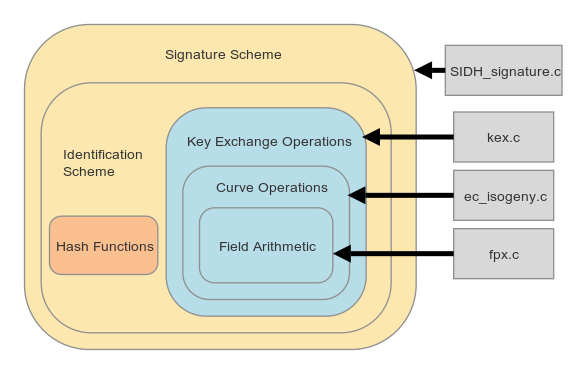
\includegraphics[scale=0.7]{fullmapwcurve.png} % e.g. insert ./image for image.png in the working directory, adjust scale as necessary
\caption{Relationship between SIDH based signatures \& the Yoo et al. fork of the SIDH C library}
\label{fig:fullmap} % insert suitable label, this is used to refer to a fig from within the text as shown above
\end{figure}

\noindent
\emph{Parallelizing Signatures}. Recall now the construction of \textbf{Sign} and \textbf{Verify} from Section \ref{sec:sigsbackground}. The sign procedure requires running $2\lambda$ distinct instances of the underlying key exchange protocol, after which these instances are reproduced in \textbf{Verify} to check for their validity. It is clear that, because every $2\lambda$ iteration of \textbf{Sign} and \textbf{Verify} are entirely independent of each other, these procedures present themselves as embarrassingly parallel.\footnote{in the field of high performance computing, a problem that is trivially parallizable is often referred to as \emph{embarrassingly} parallizable.}

This parallelization approach was exactly the one taken by Yoo et al. in their C implementation. Refer again to the \code{SIDH\_signature.c} functions outlined in Figure \ref{fig:sigfuncs}: \code{isogey\_sign} acts as the entry point for \textbf{Sign} and spawns a POSIX thread for every instance of the procedure's for-loop. So now, in parallel, every thread spawned by \code{isogeny\_sign} makes a call to \code{sign\_thread}, which in turn performs \bob's interaction with \randall. This is illustrated in Figure \ref{fig:parallelcall}. Verification proceeds analogously; \code{isogeny\_verify} is executed and spawns POSIX threads executing \code{verify\_thread} until all $2\lambda$ iterations are complete. $\lambda$ here denotes the security level in bits (128 by default in SIDH), and so 248 threads are spawned in both \code{sign\_thread} and \code{verify\_thread}.

\begin{figure}
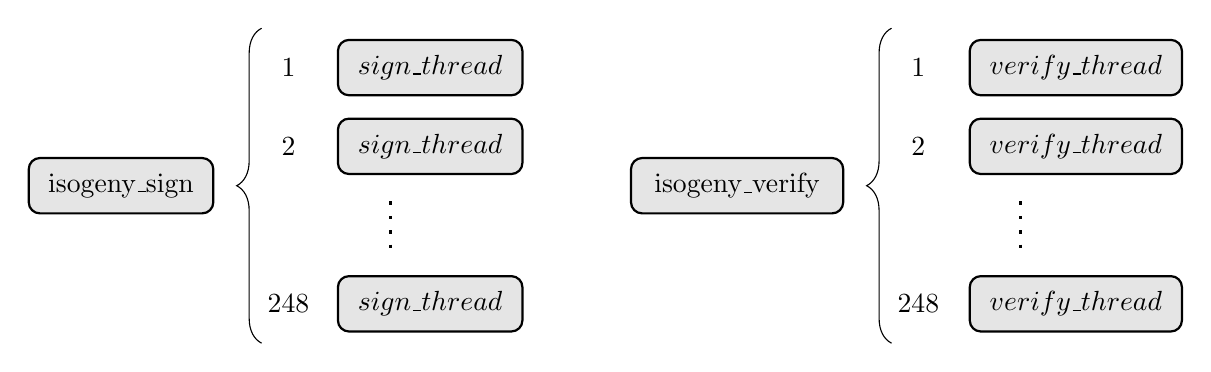
\begin{tikzpicture}
	[scale=1, auto,
		block/.style={
		  rectangle,
		  draw=black,
		  thick,
		  fill=gray!20,
		  text width=6em,
		  align=center,
		  rounded corners,
		  minimum height=2em
		},
		block1/.style={
		  rectangle,
		  draw=black,
		  thick,
		  fill=gray!20,
		  text width=7em,
		  align=center,
		  rounded corners,
		  minimum height=2em
		}
	]
	\begin{scope}[xshift=0cm]
		\draw (2.5,4.5) node[block] {$\code{sign\_thread}$};
		\draw (0.7, 4.5) node {1};
		\draw (2.5,3.5) node[block] {$\code{sign\_thread}$};
		\draw (0.7, 3.5) node {2};
		\draw[very thick, loosely dotted] (2,2.8) -- (2,2.1) node {};
		\draw (2.5,1.5) node[block] {$\code{sign\_thread}$};
		\draw (0.7, 1.5) node {248};

		\draw [decorate,decoration={brace,amplitude=9pt},xshift=-4pt,yshift=0pt] (0.5,1) -- (0.5,5.0) node [black,midway,xshift=-0.6cm,block] {\code{isogeny\_sign}};
	\end{scope}
	\begin{scope}[xshift=8cm]
		\draw (2.7,4.5) node[block1] {$\code{verify\_thread}$};
		\draw (0.7, 4.5) node {1};
		\draw (2.7,3.5) node[block1] {$\code{verify\_thread}$};
		\draw (0.7, 3.5) node {2};
		\draw[very thick, loosely dotted] (2,2.8) -- (2,2.1) node {};
		\draw (2.7,1.5) node[block1] {$\code{verify\_thread}$};
		\draw (0.7, 1.5) node {248};

		\draw [decorate,decoration={brace,amplitude=9pt},xshift=-4pt,yshift=0pt] (0.5,1) -- (0.5,5.0) node [black,midway,xshift=-0.6cm,block1] {\code{isogeny\_verify}};
	\end{scope}
\end{tikzpicture}
\caption{The implementations of \textbf{Sign} and \textbf{Verify}, divided into serial segments \code{isogeny\_sign} and \code{isogeny\_verify} and then parallel segments \code{sign\_thread} and \code{verify\_thread}.}
\label{fig:parallelcall}
\end{figure}

And so, there are two settings in which the same sequence of operations will be carried out $248$ times in parallel. This means that we need only one occurance of an $\mathbb{F}_{p^2}$ inversion in either \code{sign\_thread} or \code{verify\_thread} to be able to fill a element batch of size $248$, suitable for partial batched inversion.

Costello et al. have concisely outlined many of the \sidh isogeny and point-wise functions in Table 1 of \cite{effalg}. Examinig this Figure, we note that there are only three candidate functions containing element inversion calls: \code{j\_inv}, \code{inv\_4\_way}, and \code{get\_A}. The fact that so few functions require inversions is, again, thanks to the design decisions outlined in Section \ref{subsec:design}.\\

\noindent
\code{j\_inv} is a function returning the $j$-invariant of a curve which is used in the derivation of the shared secret. If we refer back to our definitions of \code{Sign} and \code{Verify} (Algorithms 9 and 10, respectively) we note that \code{Sign} contains a call to \code{SecretAgreement\_B} in every iteration of its for-loop. Similarly, \code{Verify} contains a call to \code{SercretAgreement\_A} in roughly half of the iterations of its for-loop, and a call to \code{SecretAgreement\_B} in the remaining iterations. This totals to $248$ secret agreement computations in both signature signing and verifying procedures. This means that somewhere in the exeuction flow of \code{isogney\_sign} and \code{isogeny\_verify} there are calls to these secret agreement functions, illustrating the presence of 1 \code{j\_inv} function call (and by extension, 1 field inversion,) in every signing and verification thread.\\

\noindent
\code{inv\_4\_way} is a function which takes 4 $\mathbb{F}_{p^2}$ elements and returns each elements inversion by means of calculating only one inversion (via the same method outlined by \textbf{BatchedInversion}). This function is used in the key generation to process to invert the Z-values of the public key curve elements; $\phi(P)$, $\phi(Q)$, and $\phi(P-Q)$), so that they can be converted from projective to affine representation. Because every \code{sign\_thread} execution represents \bob's key exchange with a distinct and random \randall, \code{KeyGeneration\_A} must be called in each thread to generate \randall's public and private keys. This results in another candidate batch of size 248 for batched partial inversion.\\

\noindent
\code{get\_A}, while containing an extension field inversion, does not arise in the execution flow of the signature scheme.\\

In Figure \ref{fig:threadcallgraph} we illustrate a heavily simplified call-graph for the \code{sign\_thread} and \code{verify\_thread}, demonstrating where in the execution pipeline \code{j\_inv} and \code{inv\_4\_way} occur. The reader may suspect that, in \code{sign\_thread} for example, the inversions in \code{SecretAgreement\_B} and \code{KeyGeneration\_A} could be batched together to form a batch of 512 elements and to reduce the total number of inversions in \code{isogeny\_sign} to one. This is not possible, however, because the valid execution of \code{SecretAgreement\_B} relies on information returned by \code{KeyGeneration\_A}, and so these inversions must occur sequentially.

\begin{figure}[!h]
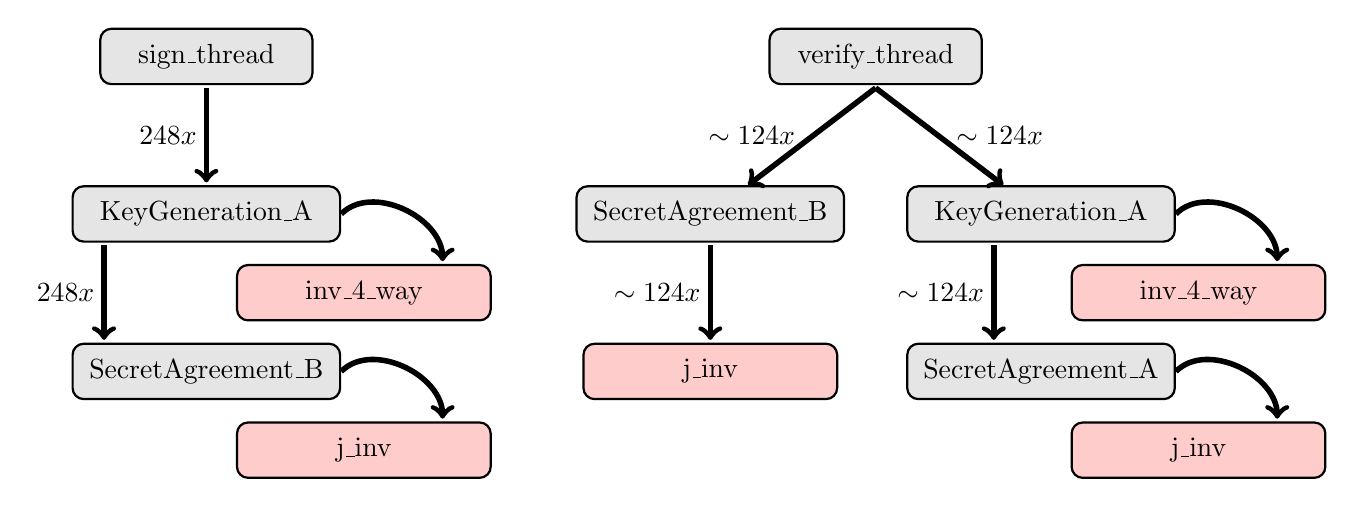
\begin{tikzpicture}
    [auto,
    block/.style={
      rectangle,
      draw=black,
      thick,
      fill=gray!20,
      text width=7em,
      align=center,
      rounded corners,
      minimum height=2em
    },
    block1/.style={
      rectangle,
      draw=black,
      thick,
      fill=gray!20,
      text width=9em,
      align=center,
      rounded corners,
      minimum height=2em
    },
	block2/.style={
      rectangle,
      draw=black,
      thick,
      fill=red!20,
      text width=8.5em,
      align=center,
      rounded corners,
      minimum height=2em
    },
    line/.style={
      draw,thick,
      -latex',
      shorten >=2pt
    },
    cloud/.style={
      draw=red,
      thick,
      ellipse,
      fill=red!20,
      minimum height=1em
    }
  ]
    \draw (1,-2) node[block] (A) {\code{sign\_thread}};
	\draw (9.5,-2) node[block] (B) {\code{verify\_thread}};
    \path (1,-4) node[block1] (C) {\code{KeyGeneration\_A}}
		  (1,-6) node[block1] (D) {\code{SecretAgreement\_B}}
		  (11.6,-4) node[block1] (E) {\code{KeyGeneration\_A}}
          (11.6,-6) node[block1] (F) {\code{SecretAgreement\_A}}
		  (7.4,-4) node[block1] (G) {\code{SecretAgreement\_B}};
	\draw (3,-7) node[block2] (H) {\code{j\_inv}};
	\draw (3,-5) node[block2] (I) {\code{inv\_4\_way}};
	\draw (7.4,-6) node[block2] (J) {\code{j\_inv}};
	\draw (13.6,-5) node[block2] (K) {\code{inv\_4\_way}};
	\draw (13.6,-7) node[block2] (L) {\code{j\_inv}};
	\draw[->, line width=2.0] (1,-2.4) -- (1,-3.6) node[right] {};
		\draw (1, -3) node[left] (LABEL1) {$248x$};
	\draw[->, line width=2.0] (9.5,-2.4) to (E) node[above] {};
		\draw (8.6, -3) node[left] (LABEL4) {$\sim124x$};
	\draw[->, line width=2.0] (9.5,-2.4) to (G) node[right] {};
		\draw (10.4, -3) node[right] (LABEL5) {$\sim124x$};
	\draw[->, line width=2.0] (-0.3,-4.4) -- (-0.3,-5.6) node {};
		\draw (-0.3, -5) node[left] (LABEL6) {$248x$};
	\draw[->, line width=2.0] (7.4,-4.4) -- (7.4,-5.6) node {};
		\draw (7.4, -5) node[left] (LABEL7) {$\sim124x$};
	\draw[->, line width=2.0] (11,-4.4) -- (11,-5.6) node {};
		\draw (11, -5) node[left] (LABEL8) {$\sim124x$};
	\draw[->, line width=2.0] (C.east) to [in=90] (4,-4.6);
	\draw[->, line width=2.0] (D.east) to [in=90] (4,-6.6);
	\draw[->, line width=2.0] (E.east) to [in=90] (14.6,-4.6);
	\draw[->, line width=2.0] (F.east) to [in=90] (14.6,-6.6);

\end{tikzpicture}
\caption{The execution flow of \code{sign\_thread} and \code{verify\_thread} as originally implemented by Yoo et al.}
\label{fig:threadcallgraph}
\end{figure}

To enable batching across execution instances of \code{j\_inv} and \code{inv\_4\_way}, we've supplied new functions \code{j\_inv\_batch} and \code{inv\_4\_way\_batch}. These functions, upon reaching what were originally $\mathbb{F}_{p^2}$ inversions (calls to \code{fp2inv751\_mont}), add their elements that are awaiting inversion to a buffer. Once the buffer of elements has reached its predefined capacity, the final thread to add its element executes \code{pb\_inv} on the buffer. Each thread thereafter, having kept track of where in the buffer they entered their element, retrieves their now inverted element from the buffer returned by \code{pb\_inv}.

\begin{figure}[!h]
\label{fig:batchcallgraph}
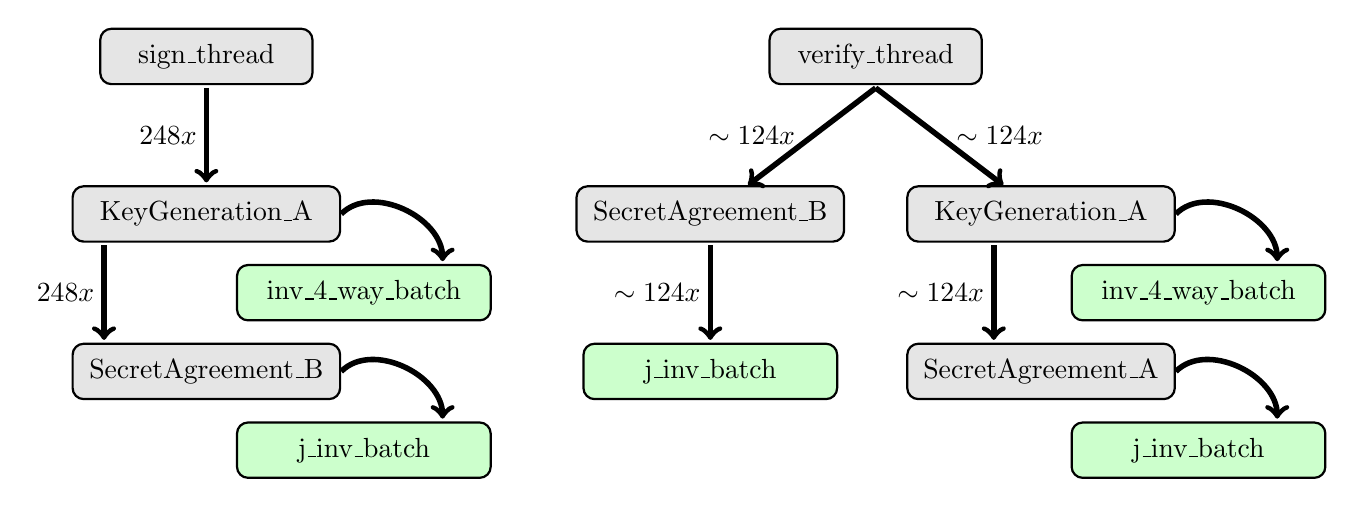
\begin{tikzpicture}
    [auto,
    block/.style={
      rectangle,
      draw=black,
      thick,
      fill=gray!20,
      text width=7em,
      align=center,
      rounded corners,
      minimum height=2em
    },
    block1/.style={
      rectangle,
      draw=black,
      thick,
      fill=gray!20,
      text width=9em,
      align=center,
      rounded corners,
      minimum height=2em
    },
	block2/.style={
      rectangle,
      draw=black,
      thick,
      fill=green!20,
      text width=8.5em,
      align=center,
      rounded corners,
      minimum height=2em
    },
    line/.style={
      draw,thick,
      -latex',
      shorten >=2pt
    },
    cloud/.style={
      draw=red,
      thick,
      ellipse,
      fill=red!20,
      minimum height=1em
    }
  ]

	\draw (1,-2) node[block] (A) {\code{sign\_thread}};
	\draw (9.5,-2) node[block] (B) {\code{verify\_thread}};
	\path (1,-4) node[block1] (C) {\code{KeyGeneration\_A}}
		  (1,-6) node[block1] (D) {\code{SecretAgreement\_B}}
		  (11.6,-4) node[block1] (E) {\code{KeyGeneration\_A}}
		  (11.6,-6) node[block1] (F) {\code{SecretAgreement\_A}}
		  (7.4,-4) node[block1] (G) {\code{SecretAgreement\_B}};
	\draw (3,-7) node[block2] (H) {\code{j\_inv\_batch}};
	\draw (3,-5) node[block2] (I) {\code{inv\_4\_way\_batch}};
	\draw (7.4,-6) node[block2] (J) {\code{j\_inv\_batch}};
	\draw (13.6,-5) node[block2] (K) {\code{inv\_4\_way\_batch}};
	\draw (13.6,-7) node[block2] (L) {\code{j\_inv\_batch}};
	\draw[->, line width=2.0] (1,-2.4) -- (1,-3.6) node[right] {};
		\draw (1, -3) node[left] (LABEL1) {$248x$};
	\draw[->, line width=2.0] (9.5,-2.4) to (E) node[above] {};
		\draw (8.6, -3) node[left] (LABEL4) {$\sim124x$};
	\draw[->, line width=2.0] (9.5,-2.4) to (G) node[right] {};
		\draw (10.4, -3) node[right] (LABEL5) {$\sim124x$};
	\draw[->, line width=2.0] (-0.3,-4.4) -- (-0.3,-5.6) node {};
		\draw (-0.3, -5) node[left] (LABEL6) {$248x$};
	\draw[->, line width=2.0] (7.4,-4.4) -- (7.4,-5.6) node {};
		\draw (7.4, -5) node[left] (LABEL7) {$\sim124x$};
	\draw[->, line width=2.0] (11,-4.4) -- (11,-5.6) node {};
		\draw (11, -5) node[left] (LABEL8) {$\sim124x$};
	\draw[->, line width=2.0] (C.east) to [in=90] (4,-4.6);
	\draw[->, line width=2.0] (D.east) to [in=90] (4,-6.6);
	\draw[->, line width=2.0] (E.east) to [in=90] (14.6,-4.6);
	\draw[->, line width=2.0] (F.east) to [in=90] (14.6,-6.6);

\end{tikzpicture}
\caption{The execution flow of \code{sign\_thread} and \code{verify\_thread} when run with inversion batching enabled}
\end{figure}

To properly implement \code{pb\_inv} in these functions, we modify every function along the call stack leading up to \code{j\_inv} and \code{inv\_4\_way}: \code{SecretAgreement\_A}, \code{SecretAgreement\_B}, and \code{KeyGeneration\_A}. Our modifications allow these functions to optionally pass a C struct we've defined which holds all of the information necessary for a successfull execution of \code{pb\_inv}. We refer to this structure as \code{batch\_struct}, and it holds the following: an integer \code{batchSize} denoting the number of elements in the batch, an integer \code{cntr} which tracks how many elements are currently in the batch (and is invariably less than or equal to \code{batchSize}), an \code{f2elm\_t} buffer \code{invArray} for storing the elements to be inverted, and an \code{f2elm\_t} buffer \code{invDest} for storing the inversion results.

Once one of the aforementioned \code{kex.c} functions reaches its call to either \code{j\_inv} or \code{inv\_4\_way}, the function checks whether the \code{batch\_struct} it has been passed is \code{NULL}. If the \code{batch\_struct} is defined, the call to \code{j\_inv} or \code{inv\_4\_way} is replaced with a call to \code{j\_inv\_batch} or \code{inv\_4\_way\_batch}, respectively.

A mutex lock can also be found in the \code{batch\_struct}, allowing \code{j\_inv} and \code{inv\_4\_way} to increment the size of the batch safely across threads. Each thread performs the following as it approaches the inversion call:
\begin{enumerate}
\item acquire the mutex lock
\item add element to be inverted to \code{invArray}
\item store the current value of \code{cntr} locally
\item increment \code{cntr}
\item release the lock
\end{enumerate}

A semaphore has also been included in \code{batch\_struct}, the function of which is to ensure that each thread knows to wait until the batch has been filled (248 elements in the signing case, ~128 in the verification cases) before it attempts to access its inverted element. If the locally stored \code{cntr} is less than \code{batchSize}, the current thread waits on the semaphore. If the locally stored \code{cntr} is equal to \code{batchSize}, this implies the current thread is the last to add its element - this thread then carries out execution of \code{pb\_inv} and upon completion posts the sempahore. After the semaphore has been posted, all other threads are able to resume execution and retrieve their now inverted elements.\\

\begin{center}
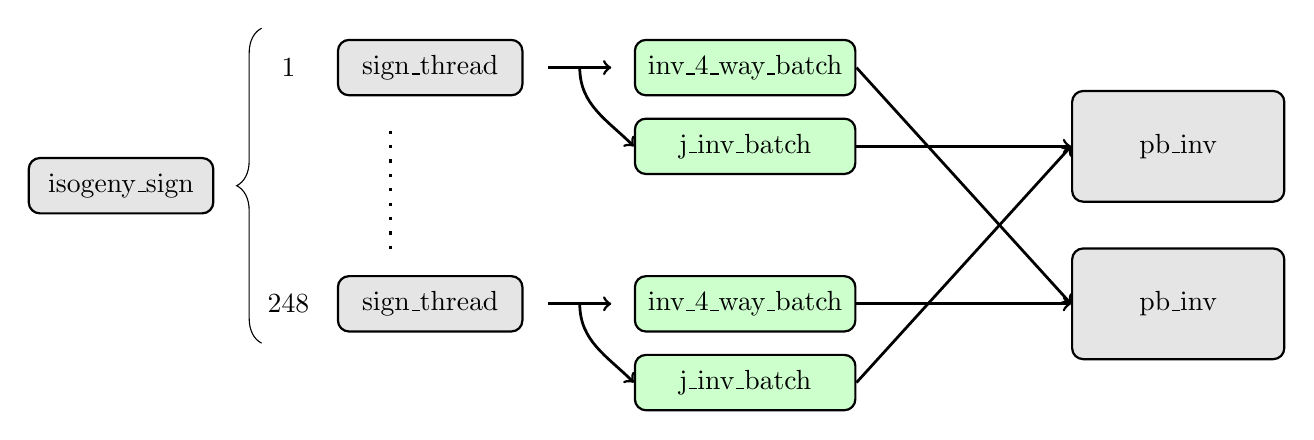
\begin{tikzpicture}
	[scale=1, auto,
		block/.style={
		  rectangle,
		  draw=black,
		  thick,
		  fill=gray!20,
		  text width=6em,
		  align=center,
		  rounded corners,
		  minimum height=2em
		},
		blockgreen/.style={
		  rectangle,
		  draw=black,
		  thick,
		  fill=green!20,
		  text width=7.3em,
		  align=center,
		  rounded corners,
		  minimum height=2em
		},
		batchblock/.style={
		  rectangle,
		  draw=black,
		  thick,
		  fill=gray!20,
		  text width=7em,
		  align=center,
		  rounded corners,
		  minimum height=4em
		}
	]
	\draw (2.5,4.5) node[block] {\code{sign\_thread}};
	\draw[->, line width=1.0] (4,4.5) -- (4.8,4.5) node {};
	%\draw [decorate,decoration={brace,amplitude=9pt},xshift=-4pt,yshift=0pt] (4.7,3.2) -- (4.7,5.7) node [black,midway,xshift=-0.6cm,block] {\code{sign\_thread}};
	\draw (6.5,3.5) node[blockgreen] (JINV1) {\code{j\_inv\_batch}};
	\draw (6.5,4.5) node[blockgreen] (INV1) {\code{inv\_4\_way\_batch}};
	\draw (0.7, 4.5) node {1};

	\draw[very thick, loosely dotted] (2,3.7) -- (2,2.2) node {};

	\draw (2.5,1.5) node[block] {\code{sign\_thread}};
	\draw[->, line width=1.0] (4,1.5) -- (4.8,1.5) node {};
	%\draw [decorate,decoration={brace,amplitude=9pt},xshift=-4pt,yshift=0pt] (4.7,0.3) -- (4.7,2.8) node [black,midway,xshift=-0.6cm,block] {\code{sign\_thread}};
	\draw (6.5,0.5) node[blockgreen] (JINV2) {\code{j\_inv\_batch}};
	\draw (6.5,1.5) node[blockgreen] (INV2) {\code{inv\_4\_way\_batch}};
	\draw (0.7, 1.5) node {248};

	\draw[->, line width=1.0] (4.4,4.5) to [out=-90] (JINV1.west);
	\draw[->, line width=1.0] (4.4,1.5) to [out=-90] (JINV2.west);

	\draw [decorate,decoration={brace,amplitude=9pt},xshift=-4pt,yshift=0pt] (0.5,1) -- (0.5,5.0) node [black,midway,xshift=-0.6cm,block] {\code{isogeny\_sign}};

	\draw (12,3.5) node[batchblock] (BATCH1) {\code{pb\_inv}};
	\draw (12,1.5) node[batchblock] (BATCH2) {\code{pb\_inv}};

	\draw[->, line width=1.0] (JINV1.east) to (BATCH1.west) node {};
	\draw[->, line width=1.0] (JINV2.east) to (BATCH1.west) node {};
	\draw[->, line width=1.0] (INV1.east) to (BATCH2.west) node {};
	\draw[->, line width=1.0] (INV2.east) to (BATCH2.west) node {};
\end{tikzpicture}
\end{center}

C code for all of these functions (with comparable differences highlighted) can be found in Appendix \ref{app:functions}.

\section{Results}

Our results come in several forms. First, there are the execution-time results of \code{pb\_inv}, compared with plain batching and unbatched inversions. Measurements of this first type are gathered in a general $\mathbb{F}_{p^2}$ environment constructed using the NTL C++ library. This allows us to meaure how the performance of \code{pb\_inv} compares with other approaches for arbitrarily sized moduli. These numbers can be found in Figures \ref{fig:moduli100} and \ref{fig:moduli1000}, and are measured in seconds. The benchmarks were taken on a single-core 1.3GHz AMD processor.

\begin{figure}[!h]
\begin{center}
\begin{tabular}{@{}llll@{}}
	\toprule
	Modulus Size & Regular Batch & \code{pb\_inv} & Unbatched \\
	\midrule
	32 & 0.351996 & 0.13946 & 0.159744\\
	64 & 0.335376 & 0.132932 & 0.167551\\
	128 & 0.356995 & 0.150744 & 0.299575\\
	256 & 0.748303 & 0.207973 & 0.486726\\
	512 & 0.655977 & 0.34409 & 0.886866\\
	1024 & 1.49688 & 0.762736 & 1.83442\\
	2048 & 3.44086 & 2.07405 & 4.39554\\
	\bottomrule
\end{tabular}
\end{center}
\caption{Execution time in seconds for 100 field element inversions using various techniques and modulus sizes (measured in seconds)}
\label{fig:moduli100}
\end{figure}

\begin{figure}[!h]
\begin{center}
\begin{tabular}{@{}llll@{}}
	\toprule
	Modulus Size & Regular Batch & \code{pb\_inv} & Unbatched \\
	\midrule
	32 & 3.45507 & 1.35421 & 1.51127\\
	64 & 3.4481 & 1.32611 & 1.61707\\
	128 & 3.64458 & 1.54956 & 2.95078\\
	256 & 7.00599 & 2.18369 & 4.80218\\
	512 & 6.563 & 3.39861 & 8.87935\\
	1024 & 14.8953 & 7.90045 & 18.3234\\
	2048 & 36.216 & 22.2085 & 42.616\\
	\bottomrule
\end{tabular}
\end{center}
\caption{Execution time in seconds for 1000 field element inversions using various techniques and modulus sizes (measured in seconds)}
\label{fig:moduli1000}
\end{figure}

The reader will note that the scale factor on performance as modulus size increases is significantly lower for \code{pb\_inv} than it is for other approaches. This is important because, as the computational power of adversaries increases, modulus sizes increase in order to ensure that compromising secret keys via a brute-force attack remains adequately difficult.

Also worth noting is how the non-partial batching algorithm performs poorly when the modulus is small. This could be an indication that for small modulus N, multiplications quickly approach the computational cost of inversions for extension field elements.\\

\noindent
We also measure the improvement in the performance of signature signing and verifying procedures offered by the inclusion of the batched partial inversion mechanism. Figure \ref{fig:batchgains} provides benchmarks for KeyGen, Sign, and Verify procedures with both batched partial inversion implemented (in the previously mentioned locations) and not implemented. All benchmarks are averages computed from 100 randomized sample runs. These results are measured in clock cycles and run on a quad-core Intel i5-8250U 1.6GHz processor.\\

\begin{figure}
\begin{center}
\begin{tabular}{@{}lllll@{}}
	\toprule
	Procedure & Without Batching & With Batching\\
	\midrule
	KeyGen & 84,499,270 & 84,499,270\\
	Signature Sign & 4,950,023,141.65 & 4,552,062,482.520\\
	Signature Verify & 3,466,703,991.09 & 3,173,340,239.461\\
	\bottomrule
\end{tabular}
\end{center}
\caption{Performance comparisons of signature subroutines run with and without batching.}
\label{fig:batchgains}
\end{figure}

With inversion batching turned on we notice a ${\sim}8$\% performance increase for both signature signing and verification.\\
